\documentclass{standalone}

\usepackage{graphicx}

\usepackage{tikz}

\usetikzlibrary{positioning}
\usetikzlibrary{arrows.meta}
\usetikzlibrary{calc}

\begin{document}

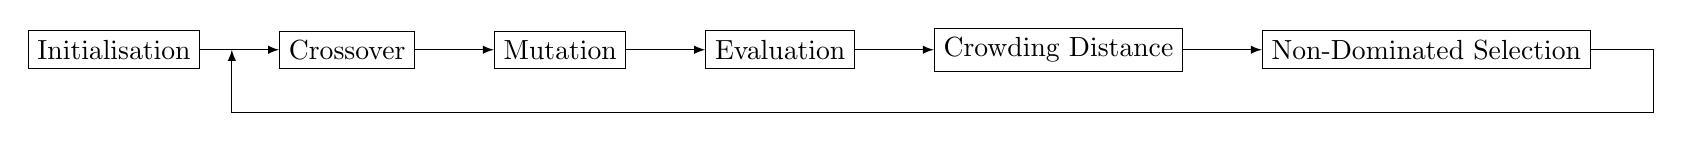
\begin{tikzpicture}[
    block/.style={rectangle, draw=black, fill=white},
]
    \node[block] (B1) [] {Initialisation};
    \node[block] (B2) [right=of B1] {Crossover};
    \node[block] (B3) [right=of B2] {Mutation};
    \node[block] (B4) [right=of B3] {Evaluation};
    \node[block] (B5) [right=of B4] {Crowding Distance};
    \node[block] (B6) [right=of B5] {Non-Dominated Selection};

    \draw[-latex] (B1.east) -- (B2.west);
    \draw[-latex] (B2.east) -- (B3.west);
    \draw[-latex] (B3.east) -- (B4.west);
    \draw[-latex] (B4.east) -- (B5.west);
    \draw[-latex] (B5.east) -- (B6.west);

    \draw[-latex] (B6.east) -| ($(B6.east)+(0.8,-0.8)$) -| ($(B1.east)+(0.4,-0.8)$) -- ($(B1.east)+(0.4,0)$);

\end{tikzpicture}

\end{document}